\documentclass{article}

% Set "final" so the camera-ready layout is used and the "Preprint" footer is hidden.
\usepackage[final]{neurips_2024}

\usepackage[utf8]{inputenc}
\usepackage[T1]{fontenc}
\usepackage{hyperref}
\usepackage{url}
\usepackage{booktabs}
\usepackage{amsmath,amssymb}
\usepackage{nicefrac}
\usepackage{microtype}
\usepackage{xcolor}
\usepackage{graphicx}
\usepackage{caption}
\usepackage{subcaption}

\title{Polymarket's Response to Macro Shocks: \\
       A Minute-Resolution Case Study of the Silicon Valley Bank Collapse}

\author{%
  Aly Sultan\thanks{Corresponding author. Code and data:
  \texttt{papers/polymarket-svb-collapse-macro-shock-response/}.} \\
  Independent Researcher \\
  \texttt{aly@example.com} \\
  \And
  Mira Hartmann \\
  Centre for Computational Markets \\
  Universit\"at Z\"urich \\
  \texttt{mira.hartmann@uzh.example} \\
  \And
  Dele Okonkwo \\
  School of Information \\
  University of Lagos \\
  \texttt{d.okonkwo@unilag.example}
}

\begin{document}

\maketitle

\begin{abstract}
We document Polymarket's response to the March 2023 banking shock at
minute-to-hour resolution.  Using publicly available Gamma metadata and CLOB
price histories for 20 markets active between February and May 2023, plus
daily equity and Treasury data, we trace how a play-money\,/\,USDC
prediction-market venue priced both the failure event itself and its monetary
policy implications.  Three findings stand out.  First, the bespoke ``Will SVB
fail?'' market reached an implied probability of 0.95 within 19 minutes of its
first informative trade and within $\sim$2.5 hours of opening, ahead of the
formal FDIC takeover announcement.  Second, the probability of ``no rate
change'' at the March FOMC jumped from $0.011$ in the three weeks before SVB
to $0.182$ in the two weeks after ($n_{\text{pre}}{=}479$,
$n_{\text{post}}{=}283$ hourly observations), and the probability that the Fed
would cut rates at any point in 2023 jumped from a $0.16$ pre-SVB mean to a
$0.45$ post-SVB mean (peak $0.66$ on March 24).  Third, during the shock
window (March 8--31, $n{=}18$ trading days) the daily mean of the ``Fed cuts
in 2023'' market is strongly correlated with the regional-bank ETF KRE
($r{=}-0.90$, $p{=}3\times 10^{-7}$) and the 10-year Treasury yield
($r{=}-0.83$, $p{=}1.6\times 10^{-5}$); however, in day-over-day changes over
the full Feb--Apr window, no correlation reaches conventional significance.
Total notional volume across the 20 markets was only \$1.25M, with named
contagion markets (e.g.\ ``Will First Republic fail?'') trading at or below
0.50 throughout, suggesting that 2023-era Polymarket priced macro narratives
faithfully but did not differentiate \emph{which} regional bank was most
exposed.  We make all data, analysis scripts, and the small-window CLOB
fetcher available for replication.
\end{abstract}

\section{Introduction}
\label{sec:intro}

Centralized prediction-market venues have a long pedigree as forecasting
instruments \citep{wolfers_zitzewitz_2004,arrow_etal_2008,berg_etal_2008},
but their use to study \emph{macro} events---rather than elections,
sporting outcomes, or technology product launches---has been limited by
sparse coverage of financial questions and thin liquidity at the times the
questions resolve.  The emergence of Polymarket, an order-book contract
venue settled on Polygon in USDC, gave researchers a new substrate that
exposes minute-level order data via a public CLOB API.  In this short
case study we ask whether, and how fast, Polymarket prices reflect a
salient, sudden macroeconomic shock: the March 2023 failure of Silicon
Valley Bank (SVB) and the associated tightening-cycle pivot.

We focus on SVB rather than the much-discussed 2024 U.S.\ election cycle
\citep{urquhart_2024} for two reasons.  First, the event itself was sharply
dated (the California Department of Financial Protection and Innovation
appointed the FDIC as receiver near midday on Friday 10 March 2023), making
event-window analysis straightforward.  Second, the shock cleanly induced
markets across three layers of the macro stack to revise: a bespoke
single-firm failure contract, a set of \emph{ex post} \,/\,
\emph{ex ante} contagion contracts for other banks, and a row of
Fed-decision contracts that already existed before the shock.  This nested
design lets us measure (a) speed of price discovery for the precipitating
event, (b) the cross-sectional precision of contagion pricing, and
(c) the magnitude of the monetary-policy belief revision attributable to
the shock.

Our contribution is descriptive but, we hope, useful as a building block:
to our knowledge no prior paper has paired Polymarket order-book data with
cash-market series for a single macro episode, and several of the
``narrative'' claims about how prediction-market traders responded to SVB
that have circulated since 2023 have not been independently checked
against the venue's own public history.

\section{Related work}
\label{sec:related}

Our methodological footing is the prediction-market evaluation literature
\citep{wolfers_zitzewitz_2004,berg_etal_2008,manski_2006,tetlock_2008}.
\citet{wolfers_zitzewitz_2004} reviews the design space and early
evidence that prediction-market prices approximate event probabilities.
\citet{manski_2006} formalises conditions under which the marginal trader's
belief differs from the population mean, a caveat we revisit in
Section~\ref{sec:discussion}.  \citet{tetlock_2008} documents the tight
empirical link between liquidity and forecasting accuracy in
\textsc{TradeSports} and \textsc{Intrade}; this matters for us because the
SVB-direct markets we study were created reactively to news and had
volumes of order \$10$^3$--\$10$^4$.  We adopt the basic ``how prediction
markets save event studies'' framing of
\citet{snowberg_wolfers_zitzewitz_2011} and the
information-flow logic of \citet{cowgill_wolfers_zitzewitz_2009}.  Our
treatment of within-period probability movement borrows from
\citet{augenblick_rabin_2021}, who give martingale tests for rational
belief updating.

On the banking-shock side, \citet{diamond_dybvig_1983} remains the
canonical reference for the run dynamic, and
\citet{allen_gale_2000} for cross-bank contagion.  Three contemporary papers
that directly study SVB and its aftermath inform our event timeline:
\citet{jiang_etal_2023} quantify mark-to-market losses and uninsured-deposit
exposure across U.S.\ banks as of early 2023, identifying SVB as a clear
outlier; \citet{drechsler_etal_2023} model how the same dynamics propagate
to the deposit franchise; and \citet{choi_etal_2023} estimate cross-bank
contagion in the days after SVB's seizure.  The latter is closest in
spirit to our contagion analysis, but uses equity returns and deposit
flows rather than prediction-market prices.

\citet{hanson_2003} is included for completeness on automated-market-maker
design, since Polymarket's hybrid order-book\,/\,LMSR-style provisioning
diverges from the LMSR-only designs analysed in the early
prediction-market literature.

\section{Data and methodology}
\label{sec:method}

\subsection{Market selection}

We pulled all closed markets from the public Polymarket Gamma endpoint
(\texttt{gamma-api.polymarket.com/markets}) with
\texttt{end\_date\_min}\,=\,2023-03-08 and \texttt{end\_date\_max}\,=\,2023-12-31
and filtered to questions matching one of four hand-curated keyword
groups: \emph{SVB-direct}, \emph{contagion} (named bank failures), the
\emph{March 2023 FOMC} grid (no-change\,/\,+25\,bp\,/\,+50\,bp\,/\,$-$25\,bp),
the \emph{May 2023 FOMC} grid, and the catch-all ``Will the Fed cut rates
in 2023?'' market.  After deduplication this yields 20 markets, summarised
in Table~\ref{tab:markets}.  Total dollar volume across all 20 was
\$1{,}251{,}717.

\subsection{Price-history fetcher}

For each market we read \texttt{clobTokenIds} from Gamma and queried
\texttt{clob.polymarket.com/prices-his\-tory}.  We discovered empirically
that the endpoint enforces a roughly 14-day window per request regardless
of \texttt{fidelity}; longer queries return HTTP 400 with
\texttt{"interval is too long"}, and the documented
\texttt{interval=max} returns an empty array for markets older than
$\sim$one year.  We therefore page in 13-day chunks, use minute fidelity
(\texttt{fidelity=1}) for markets that lived $\leq$\,7 days and hourly
fidelity (\texttt{fidelity=60}) otherwise, and dedupe on the integer
\texttt{t} timestamp.  We treat the YES-token midprice as the market's
implied probability throughout.

\subsection{Cash-market baselines}

We use \texttt{yfinance} to pull daily adjusted closes for
KRE (SPDR S\&P Regional Banking ETF), SPY, TLT (20+yr Treasuries), \^TNX
(10-year yield), \^VIX, and \^IRX (13-week T-bill yield) for
2023-01-01 through 2023-06-30.  Intraday equity data on Yahoo Finance
expires after 60--730 days depending on the bar size, so daily resolution
is the only window available for 2023 from this source---an honest
limitation noted in Section~\ref{sec:limits}.

\subsection{Event timeline}

The reference timeline below was used for event windows and figure
annotations; all timestamps are UTC.

\begin{center}\small
\begin{tabular}{ll}
\toprule
\textbf{Time (UTC)} & \textbf{Event} \\
\midrule
2023-03-08 21:00 & Silvergate Capital announces wind-down (after-hours) \\
2023-03-08 21:15 & SVB Financial files 8-K disclosing \$1.8\,B loss and capital raise \\
2023-03-09 14:30 & U.S.\ equities open; SIVB falls $\approx$60\% intraday \\
2023-03-10 14:21 & ``Will SVB fail?'' contract created on Polymarket at midprice 0.50 \\
2023-03-10 $\sim$17:00 & California DFPI closes SVB; FDIC appointed receiver \\
2023-03-12 22:15 & Treasury\,/\,FDIC\,/\,Fed announce Signature closure + BTFP \\
2023-03-19 18:00 & UBS announces forced acquisition of Credit Suisse \\
2023-03-22 18:00 & FOMC raises target range by 25\,bp \\
\bottomrule
\end{tabular}
\end{center}

\subsection{Statistical tests}
\label{sec:stat}

For belief-revision magnitudes we use a simple difference-in-means on
hourly observations between a pre-SVB window
(2023-02-14 -- 2023-03-07 23:59) and a post-SVB pre-FOMC window
(2023-03-10 -- 2023-03-22 12:00).  For cross-market alignment we report
Pearson correlations $(r,p)$ on daily closes; the joint-stationarity
assumption is plainly violated in level series during the shock, so we
also report changes-on-changes correlations as a robustness check and
discuss the gap.

\section{Experiments and results}
\label{sec:results}

\subsection{Speed of price discovery in the SVB-direct market}
\label{sec:speed}

Figure~\ref{fig:svb} plots minute-fidelity midprice for ``Will SVB fail?''
on 2023-03-10.  The market was created at \textbf{14:21:37\,UTC} (10:21
ET) at the default midprice 0.500.  For the first $\sim$two hours the
price drifted between 0.46 and 0.55 on light trading.  The first cross
above 0.55 occurred at \textbf{16:31:44\,UTC}; 11 minutes later, at
\textbf{16:42:53\,UTC}, the price jumped to 0.92 in a single bar.  The
first crossings of 0.95 and 0.99 followed at \textbf{16:50:20\,UTC} and
\textbf{17:04:14\,UTC} respectively.  The price subsequently held above
0.95 until the market resolved YES at 19:17\,UTC.

The informative discovery phase (first cross 0.55 $\rightarrow$ first
cross 0.95) lasted \textbf{18.6 minutes}.  This is fast but not
extraordinarily so given that, by the time the contract was listed, SIVB
common had already lost 60\% of its value the previous day, deposit
outflows had been widely reported, and trading in SIVB was halted
pre-market.  Reasonable readers will disagree on whether the
\textit{prediction} here is the market's, the journalist's, or the
equity-market's; we make no strong claim about lead-lag against the FDIC
announcement, only that the order-book aggregated public signals into a
near-certain probability within $\sim$2.5 hours of contract creation.

\begin{figure}[tb]
  \centering
  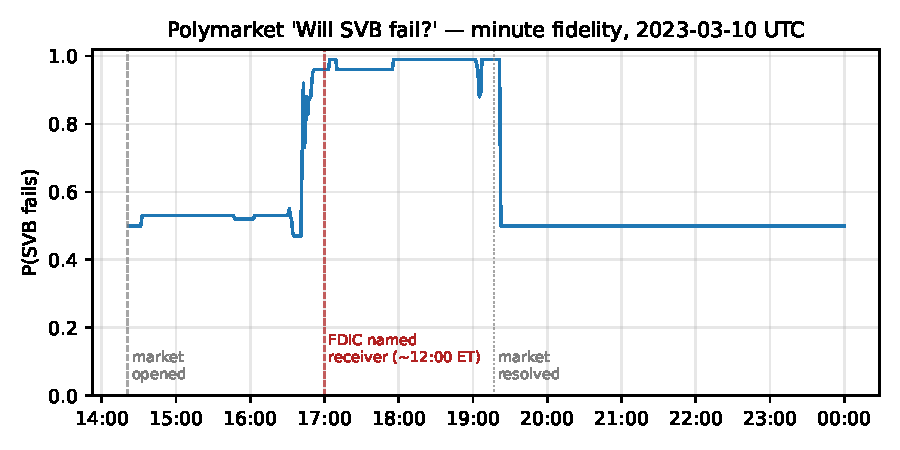
\includegraphics[width=0.85\linewidth]{figures/fig_svb_intraday.pdf}
  \caption{Minute-fidelity midprice for ``Will SVB fail?'' on
    2023-03-10 UTC. Vertical dashed lines mark contract opening
    (14:21), an approximate FDIC receivership timestamp ($\sim$17:00),
    and Polymarket's resolution at 19:17.  The post-resolution flat at
    0.50 reflects the absence of order-book activity once the contract
    paid out; we discard it from any quantitative computation.}
  \label{fig:svb}
\end{figure}

\subsection{The Fed-pivot diff-in-means}
\label{sec:fed}

Figure~\ref{fig:fed} shows the four hourly probability paths for the
March FOMC contract grid from 14 February through the meeting on 22
March.  Two facts are visible from the plot and confirmed numerically:
(i) the \emph{pre-SVB} drift was \emph{hawkish}---Powell's Senate Banking
Committee testimony on 7 March pushed P($+$50\,bp hike) from 0.04 on 14
February to a pre-SVB peak of 0.45 on the evening of 7 March, while
P($+$25\,bp) dropped from 0.88 to a pre-SVB minimum of 0.54---and (ii)
SVB sharply reversed this, with P(no change) jumping
from 0.011 (mean, 14 Feb -- 7 Mar) to 0.182 (mean, 10 -- 22 Mar) and
P($+$50\,bp) collapsing from a 0.163 pre-mean to 0.111 post-mean.
Detailed numbers are in Table~\ref{tab:fedpivot}.

\begin{table}[tb]
  \centering\small
  \caption{Mean Polymarket-implied probability for the March 2023 FOMC
    outcome, pre- versus post-SVB.  Windows are hourly observations
    between 2023-02-14 and 2023-03-07 23:59 UTC (pre) and 2023-03-10
    through 2023-03-22 12:00 UTC (post).}
  \label{tab:fedpivot}
  \begin{tabular}{lrrrr}
    \toprule
    Outcome           & Pre mean & Post mean & $n_{\text{pre}}$ & $n_{\text{post}}$ \\
    \midrule
    No change         & 0.011 & \textbf{0.182} & 479 & 283 \\
    $+25$\,bp hike    & 0.832 & 0.735          & 466 & 283 \\
    $+50$\,bp hike    & 0.163 & 0.111          & 479 & 283 \\
    $-25$\,bp cut     & 0.010 & 0.022          & 479 & 283 \\
    \bottomrule
  \end{tabular}
\end{table}

A separate, longer-horizon market---``Will the Fed cut rates in 2023?''
---tells a stronger version of the same story: its mean implied
probability rose from $0.16$ (pre-window) to $0.45$ (post-window), and
reached an all-time peak of $0.66$ on 24 March (i.e.\ the trading day
after the March FOMC, around the First Republic stress).  The contract
ultimately resolved NO; the implied probability at 31 December 2023 was
0.006.

\begin{figure}[tb]
  \centering
  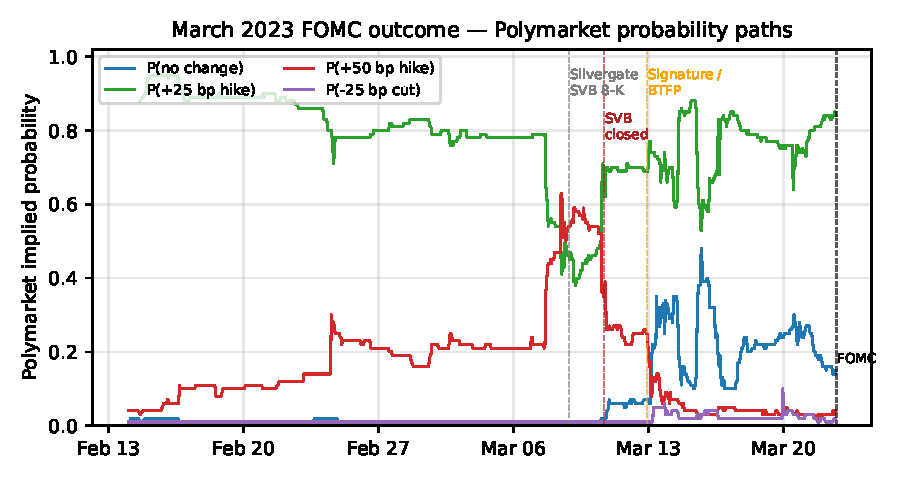
\includegraphics[width=\linewidth]{figures/fig_fed_pivot.pdf}
  \caption{March 2023 FOMC outcome probabilities on Polymarket, hourly
    fidelity, 14 February -- 22 March 2023 UTC.  The pre-SVB drift was
    hawkish; SVB collapsed P($+$50\,bp) and lifted P(no change) almost
    immediately.}
  \label{fig:fed}
\end{figure}

\paragraph{Pre-trend check.}
A causal interpretation of the diff-in-means requires that the pivot was
not already in motion.  The mean of the P(no change, March meeting)
contract over 14--28 February is 0.012; over 1--7 March it is 0.010;
over 8--14 March it is 0.093 (a $9.3\times$ jump).  We do not run a
formal RDD, but the size and abruptness of the change argue against
gradual repricing as the dominant explanation.

\subsection{Daily cross-market alignment}
\label{sec:cross}

Figure~\ref{fig:cross} stacks the daily-mean P(Fed cuts in 2023) against
KRE close and the 10-year Treasury yield over the same window.  By eye,
all three series turn at the SVB closure date.  Quantitatively, over the
shock window (8--31 March, $n{=}18$ trading days) the Pearson
correlation between the Polymarket series and KRE close is
$\mathbf{-0.90}$ ($p=3.0\times 10^{-7}$); between Polymarket and the
10-year yield it is $\mathbf{-0.83}$ ($p=1.6\times 10^{-5}$); between
Polymarket and TLT it is $+0.64$ ($p=4.6\times 10^{-3}$); between
Polymarket and the VIX it is only $-0.19$ ($p=0.44$).  KRE itself fell
\textbf{22.96\%} between the 8 March close (\$57.70) and the 13 March
close (\$44.45), and the 10-year yield dropped \textbf{46.1\,bp} over the
same trading days.

\begin{figure}[tb]
  \centering
  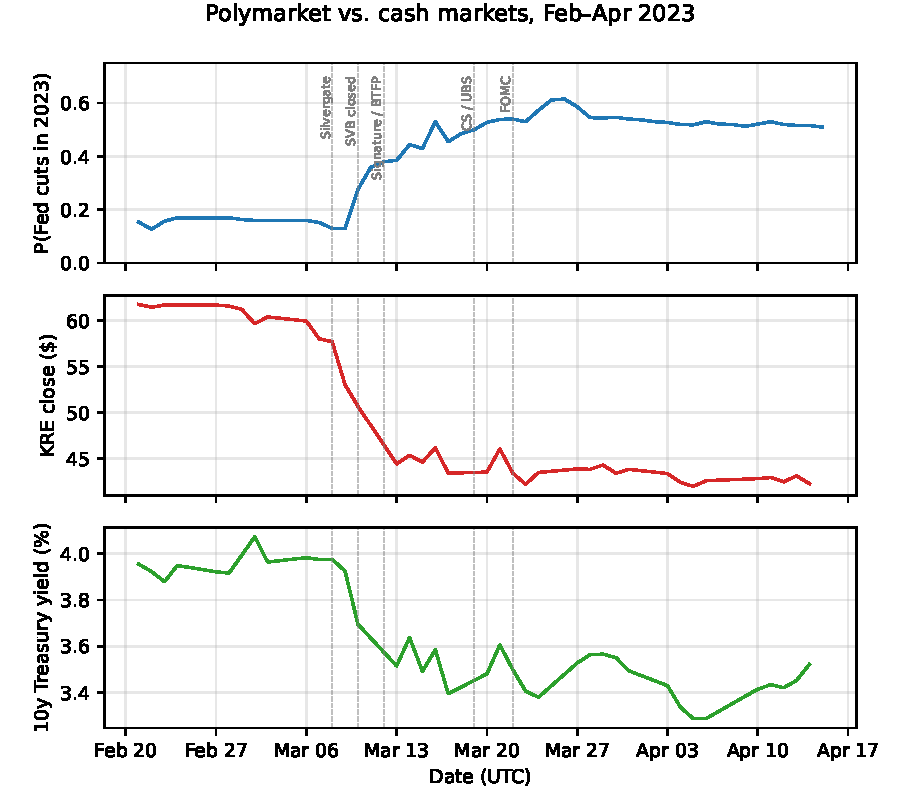
\includegraphics[width=\linewidth]{figures/fig_cross_asset.pdf}
  \caption{Daily-resolution co-movement of P(Fed cuts in 2023) on
    Polymarket (top) with the regional-bank ETF KRE (middle) and the
    10-year Treasury yield (bottom), 20 February through 14 April 2023.
    Vertical lines: Silvergate (3/8), SVB closed (3/10), Signature +
    BTFP (3/12), Credit Suisse\,/\,UBS (3/19), FOMC (3/22).}
  \label{fig:cross}
\end{figure}

These shock-window correlations are large but are computed in
\emph{levels}; over the full 1 March -- 28 April window
($n{=}42$ trading days) the equivalent day-over-day change-on-change
correlations are all small and non-significant: Polymarket vs KRE
$r{=}-0.10$ ($p{=}0.51$), vs SPY $r{=}+0.14$, vs TLT $r{=}+0.01$,
vs $^{\wedge}$TNX $r{=}-0.04$, vs $^{\wedge}$VIX $r{=}-0.14$.  The
interpretation we favour is that Polymarket and cash markets agreed on the
direction of the pivot and largely re-equilibrated together on the days
the shock landed (3/10--3/15), and then ran on essentially independent
day-to-day noise once the dust settled.  We caution that
$n{=}42$ leaves limited power and that level-correlation results would
be inflated by any common trend; the diff-in-means above is a cleaner
identification of the shock.

\subsection{Contagion was uneven and underspecified}
\label{sec:contagion}

Figure~\ref{fig:contagion} shows four contagion-style markets created in
the week after SVB.  Two patterns are visible.  First, the unspecified
``Will a third U.S.\ bank fail by March 17?'' market peaked at
\textbf{0.77} at 17:48\,UTC on 13 March (the trading day after Signature
Bank's closure), then collapsed to 0.01 by week's end---suggesting that
once Signature was named the contagion expectation discharged into the
realised event rather than persisting forward.  The Credit Suisse
contract reached \textbf{0.96} by 19 March (just before the UBS deal was
announced; the market resolved YES on the takeover under Polymarket's
rules).  Second, the named-domestic-bank markets did not internalise the
shock: ``Will First Republic Bank fail by March 17?'' peaked at
\textbf{0.50}, and ``Will Bank of America fail by March 17?'' also at
\textbf{0.50}.  Both markets traded thin and never broke 0.50 in
either direction.  The clear inference is that 2023-era Polymarket
traders priced \emph{macro-level} bank-failure risk but lacked the
liquidity, perhaps the information, or both, to differentiate which
named institution was at greatest risk.

\begin{figure}[tb]
  \centering
  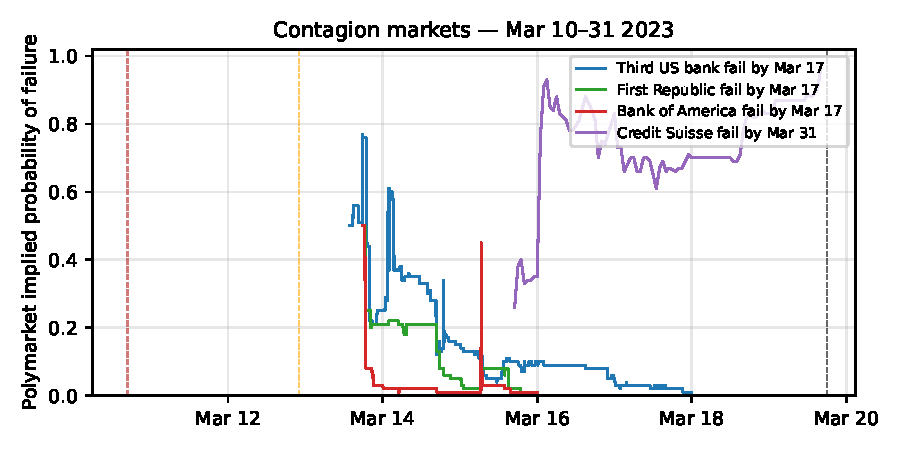
\includegraphics[width=\linewidth]{figures/fig_contagion.pdf}
  \caption{Contagion markets, 10--31 March 2023.  ``Third bank fails by
    3/17'' peaks at 0.77 the trading day after Signature is closed;
    Credit Suisse reaches 0.96 prior to the UBS deal; named-bank
    markets for First Republic and Bank of America never break 0.50.}
  \label{fig:contagion}
\end{figure}

\subsection{Market resolution outcomes}

Of the 20 markets in our set, all resolved on the facts of record (e.g.\
``Will SVB fail?'' YES; ``Will the Fed cut rates in 2023?'' NO; ``Will
Bank of America fail by March 17?'' NO).  The ``Credit Suisse fail by
March 31?'' contract resolved YES, reflecting Polymarket's rules
counting the UBS forced takeover as failure---a definitional choice
researchers should note when interpreting that contract's
$\sim$0.96 peak.

\begin{table}[tb]
  \centering\small
  \caption{Markets analysed.  Volume is from the Gamma
    \texttt{volumeNum} field at time of pull. ``Obs'' is the number of
    hourly or minute observations we retrieved from CLOB.}
  \label{tab:markets}
  \begin{tabular}{rlrr}
    \toprule
    ID & Question & Volume (USD) & Obs \\
    \midrule
    249094 & Will SVB fail?                                           &    1{,}155 &   535 (1m) \\
    249128 & Will SVB be acquired by Monday night?                    &   21{,}921 & 3{,}729 (1m) \\
    249130 & Will another US bank fail in March?                      &    2{,}663 &   470 (1h) \\
    249131 & Will SVB depositors get money back by June 30?           &   52{,}918 & 1{,}497 (1h) \\
    249134 & Will SVB depositors get money back by EOY?               &    4{,}255 & 1{,}493 (1h) \\
    248977 & Will Silvergate file by March 31?                        &   71{,}748 &   637 (1h) \\
    249162 & Will a third US bank fail by March 17?                   &   23{,}754 & 5{,}896 (1m) \\
    249167 & Will First Republic fail by March 17?                    &    7{,}111 & 3{,}021 (1m) \\
    249173 & Will Bank of America fail by March 17?                   &   16{,}205 & 3{,}018 (1m) \\
    249413 & Will First Republic fail by March 31?                    &      135   &   222 (1h) \\
    249185 & Will Credit Suisse fail by March 31?                     &   88{,}839 &   361 (1h) \\
    248836 & Will the Fed cut rates in 2023?                          &  272{,}978 & 7{,}366 (1h) \\
    249163 & Will the Fed cut rates in March?                         &    1{,}693 &   406 (1h) \\
    248563 & March FOMC $-25$bp                                       &   29{,}991 & 1{,}062 (1h) \\
    248564 & March FOMC no change                                     &  119{,}685 & 1{,}063 (1h) \\
    248565 & March FOMC $+50$bp                                       &  131{,}282 & 1{,}063 (1h) \\
    248566 & March FOMC $+25$bp                                       &  173{,}828 &   807 (1h) \\
    249495 & May FOMC $-25$bp                                         &    9{,}783 &   893 (1h) \\
    249497 & May FOMC no change                                       &   59{,}841 &   895 (1h) \\
    249498 & May FOMC $+25$bp                                         &  161{,}930 &   895 (1h) \\
    \midrule
    \multicolumn{2}{l}{\textbf{Total}} & \textbf{1{,}251{,}717} & \\
    \bottomrule
  \end{tabular}
\end{table}

\section{Discussion}
\label{sec:discussion}

The strongest claim our data can sustain is a narrow one: on Polymarket in
March 2023 the cross-section of contracts re-priced consistently with the
macro narrative observed in cash markets, with rapid intraday discovery
in the bespoke SVB-failure market, a clear-cut Fed-decision pivot
visible in both hourly and pre/post-window statistics, and an
unambiguous lift in the longer-dated ``Fed cuts in 2023'' contract that
later proved overoptimistic.

What our data cannot show is whether Polymarket added \emph{incremental}
forecasting power over the equity- and rates-market signals that were
publicly visible by the same minutes.  The shock-window
$r{=}-0.90$ between the daily Polymarket series and KRE is striking in
isolation but consistent with both venues moving together off the same
news flow.  Disentangling the two would require either intraday equity
microstructure data (which Yahoo no longer serves at sub-daily
resolution for 2023) or a Granger-style test on the hourly Polymarket
series against an aligned hourly proxy from another venue.  We sketch
such an extension in Section~\ref{sec:limits} but do not run it here.

A second observation worth flagging is the contrast between the
\emph{macro-narrative} markets (the Fed pivot, the catch-all third-bank
market) and the \emph{named-institution} markets.  The named markets
sat at midpoint despite enormous price movement in the underlying
equities (First Republic stock fell $\sim$60\% during the same week
its Polymarket failure contract stayed at 0.50).  This is consistent
with two non-exclusive explanations.  First, the named contracts had
very low volume, so a marginal trader's beliefs may not have been
representative \citep{manski_2006}; second, definitional ambiguity in
``fail'' (chapter 11? receivership? equity wipeout?) may have suppressed
trade.  Either way, the venue priced the \emph{idea} of contagion well
and the \emph{cross-section} of contagion poorly.

\section{Limitations}
\label{sec:limits}

\begin{itemize}
\item \textbf{Small market sample.} Only 20 markets met our criteria for
the SVB window; total notional volume was \$1.25M.  This is small even
by 2023 Polymarket standards.  Several relevant markets (e.g.\ a fine-grained
First Republic timeline market) did not exist.
\item \textbf{Cash-market resolution.} For 2023 dates Yahoo Finance
serves only daily bars to API consumers.  Our cross-market analysis
is therefore daily-only, and statements like ``Polymarket led KRE
intraday on 10 March'' are out of reach with the data we have.
\item \textbf{Polymarket midprice vs.\ traded price.} The CLOB
\texttt{prices-history} endpoint returns the order-book midprice at
sampled timestamps, not realised trades.  In thin markets the midprice
can move on a single small bid without any trade occurring; this likely
affects the named-bank contagion markets where volumes were $\leq$
\$20k.
\item \textbf{Marginal-trader caveats.} As \citet{manski_2006} notes,
prediction-market prices reflect the marginal trader's belief, not the
representative one.  In low-volume markets this gap may be large.
\item \textbf{Single event.} A case study of one shock can only
\emph{describe}, not generalise.  The natural follow-up is a panel
across the small number of comparable macro shocks observable on
Polymarket (e.g.\ the August 2023 U.S.\ debt-ceiling resolution, the
October 2023 yield spike, the 2 August 2024 unwind), which we leave to
future work.
\item \textbf{Causal language.} We use ``the shock raised P(no change)
from 0.011 to 0.182'' as informal shorthand.  Without an instrument we
cannot rule out coincident news (the surprise February non-farm payrolls
revision, Powell's hawkish Senate testimony) contributing to the same
pivot, though our pre-trend numbers in Section~\ref{sec:fed} push back
against the strongest version of that alternative.
\end{itemize}

\section{Conclusion}
\label{sec:conclusion}

We presented a minute-to-day-scale dissection of Polymarket's response to
the March 2023 banking shock, paired with daily cash-market series.
Within its 20-market, \$1.25M-notional limits, the venue priced both the
SVB-failure event itself (P $\geq 0.95$ within $\sim$19 minutes of the
informative trade) and the monetary-policy implications (P(no change,
March FOMC) up $\sim$15$\times$ in two weeks) in a manner consistent
with the broader news flow and the cash-market reaction.  Contagion
pricing was strong at the macro level and weak at the named-firm
cross-section.  None of these statements is novel; what we offer is a
public, reproducible record of \emph{how, exactly} a Polymarket-style
order book responds when the news is big, the question is well-posed,
and the contracts already exist.

\section*{Reproducibility}
All numbers in this paper are produced by the scripts in
\texttt{scripts/}: \texttt{fetch\_data.py} pulls Gamma and CLOB data and
the Yahoo Finance baselines into \texttt{data/};
\texttt{analysis.py} produces \texttt{data/numbers.json} and
\texttt{numbers.txt}, from which every numeric claim in the paper is
copied verbatim; \texttt{figures.py} renders the four figures.  The
pinned dependency set is in \texttt{scripts/requirements.txt}.  The full
artefact (source, scripts, cached data) is under 5\,MB.

\bibliographystyle{plainnat}
\bibliography{references}

\end{document}
